\documentclass[onecolumn]{article}
%\usepackage{url}
%\usepackage{algorithmic}
\usepackage[a4paper]{geometry}
\usepackage{datetime}
\usepackage[margin=2em, font=small,labelfont=it]{caption}
\usepackage{graphicx}
\usepackage{mathpazo} % use palatino
\usepackage[scaled]{helvet} % helvetica
\usepackage{microtype}
\usepackage{amsmath}
\usepackage{subfigure}
\usepackage{listings}
\usepackage{float}
\usepackage{color} %red, green, blue, yellow, cyan, magenta, black, white
\usepackage{graphicx}
\usepackage[font=small,labelfont=bf]{caption}
\renewcommand{\thefigure}{\arabic{section}.\arabic{figure}}
\graphicspath{ {pictures/} }
\definecolor{mygreen}{RGB}{28,172,0} % color values Red, Green, Blue
\definecolor{lightgray}{gray}{0.9}
\definecolor{mylilas}{RGB}{170,55,241}
\newcommand{\inlinecode}[2]{\colorbox{lightgray}{\lstinline[language=#1]$#2$}}


% Letterspacing macros
\newcommand{\spacecaps}[1]{\textls[200]{\MakeUppercase{#1}}}
\newcommand{\spacesc}[1]{\textls[50]{\textsc{\MakeLowercase{#1}}}}

\title{\spacecaps{Lab report: Lab 3-4 }\\
Heat transfer simulation\\\normalsize \spacesc{Modeling of Physical Systems} }

\author{Patryk Gałczyński}
%\date{\today\\\currenttime}
\date{\today}


\begin{document}

\lstset{language=Matlab,%
    %basicstyle=\color{red},
    %breaklines=true,%
    morekeywords={matlab2tikz},
    keywordstyle=\color{blue},%
    morekeywords=[2]{1}, keywordstyle=[2]{\color{black}},
    identifierstyle=\color{black},%
    stringstyle=\color{mylilas},
    commentstyle=\color{mygreen},%
    showstringspaces=false,%without this there will be a symbol in the places where there is a space
    numbers=left,%
    numberstyle={\small \color{black}},% size of the numbers
    numbersep=9pt, % this defines how far the numbers are from the text
    emph=[1]{for,end,break},emphstyle=[1]\color{red}, %some words to emphasise
    %emph=[2]{word1,word2}, emphstyle=[2]{style},    
}

\maketitle


\section{Aim}
\large
The aim of this laboratory was to simulate, visualize and analyze heat transfer process in three different materials - copper, stainless steel and aluminum with two methods.


\section{Methods}
For the laboratory purpose various tools and methods were selected to achieve good simulation results and easy in depth analysis. Simulation model has been tested against its theoretical model, its numerical stability as well as state stability after time.


\subsection{Simulation description}
This simulation considers metal plate with size of 25 centimeter by 25 centimeter which is being heated on highlighted area figure \ref{fig:plate} (which is 5 centimeters by 5 centimeters) in couple different ways. Heater area is square shaped and placed in center of the plate. 

\begin{itemize}
	\item Situation 1 - heater area (the red one) is having constant temperature during whole simulation equal to $80^{o}$ of Celsius. Outer edge has fixed temperature as well and is equal to $10^{o}$ of Celsius all the time. This situation assumes that plate is infinitely thin.
    \item Situation 2 - heater area provides constant amount of energy - 100 Wats for first 10 seconds. It is assumed that outer edge is thermally isolated from environment, that means it does not exchanges energy. This time, plate does have finite thinness. 
\end{itemize}

\begin{figure}[H]
\noindent\makebox[\textwidth]{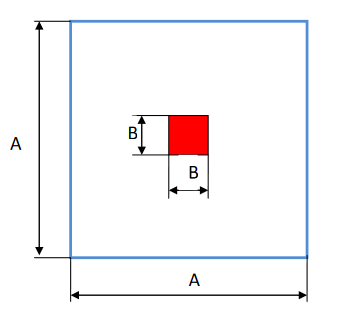
\includegraphics[]{plate}}
\caption{Metal plate that is being heated}
\label{fig:plate}
\end{figure}


\subsection{Software}
To simulate, compute and visually represent heat transfer process MATLAB software was involved.

\section{Results}
\subsection{Simulation of heat transfer phenomena code}
Following code has been used to simulate and visually represent heat transfer in two described situations. First part, which is declaration of constant values, stays the same for both situations:
\begin{lstlisting}[language=Matlab,frame=single,label={lst:autocorr},breaklines=true,caption={initial values for matlab scripts}]
% time variables
number_of_steps = 100;           % num
dt = 0.1;                        % s
dx = 0.01;                       % m
dy = 0.01;                       % m



% metal variables
K = 237;                         % W/mK
cw = 900;                        % J/kgK
ro = 2700;                       % kg/m3

% plane variables
outer_size = 25;                 % cm
inner_size = 5;                  % cm
% only these differs for different situations
outer_temp = 10;                 % C
inner_temp = 80;                 % C
small_start = (outer_size - inner_size)/2;
\end{lstlisting}

In first situation (boundary condition 1), temperature of heater area and outer boarder has to be fixed, which is done in lines 2 and 3 for initial condition and in lines 18 to 22 for every timestamp. Temperature on every point belonging to plane is calculated with formula provided in lab instruction. At the very end surface plot of last calculated state is being used to visualize final result.

\begin{lstlisting}[language=Matlab,frame=single,label={lst:autocorr},breaklines=true,caption={matlab script implementing first boundary condition}]
% assign initial plate state
plane(1:outer_size,1:outer_size,1) = outer_temp;
plane(small_start:small_start+inner_size,small_start:small_start+inner_size, 1) = inner_temp;

% iterate over time
for i = 2:number_of_steps
    % iterate over plate points
    for x = 2:outer_size-1
        for y = 2:outer_size-1
            % change plane state according to given formula
            plane(x,y,i) = ...
                plane(x,y,i-1) + ...
                (K*dt)*(plane(x+1,y,i-1) - 2*plane(x,y,i-1) + plane(x-1,y,i-1))/(cw*ro*dx*dx) + ...
                (K*dt)*(plane(x,y+1,i-1) - 2*plane(x,y,i-1) + plane(x,y-1,i-1))/(cw*ro*dy*dy);
        end
    end
    % restore initial conditions at heater area and outer edge
    plane(small_start:small_start+inner_size,small_start:small_start+inner_size, i) = inner_temp;
    plane(1,:,i) = outer_temp;
    plane(:,1,i) = outer_temp;
    plane(outer_size,:,i) = outer_temp;
    plane(:,outer_size,i) = outer_temp;

end

% plot awesome graph
[XX, YY] = meshgrid(1:outer_size,1:outer_size);
surf(XX,YY,plane(:,:,number_of_steps));
\end{lstlisting}

Result of this script execution is the following chart
\begin{figure}[H]
\noindent\makebox[\textwidth]{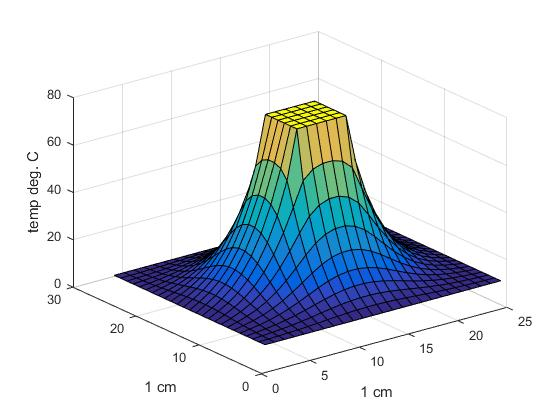
\includegraphics[scale=0.6]{first_script}}
\caption{Heat transfer for first boundary condition using copper plate after certain number of time steps}
\label{fig:plate}
\end{figure}

There are several conclusions to be made. First of all, it is clearly visible that the hottest part is always in place of heater. Secondly, area near the heater is propagating energy to its neighbors, which results in warmer area then in beginning of the simulation.

Code for second situation is mostly the same as for first one, however different parts are:
\begin{itemize}
    \item $inner\_temp = outer\_temp = 20^{o}C$
    \item in line 12 is if statement checking whether heater should be in on state.
    \item surface plot changes over time to show how temperature of plane is changing
    \item $heating\_power$ is equal to $100W$
\end{itemize}
\begin{lstlisting}[language=Matlab,frame=single,label={lst:bc2},breaklines=true,caption={matlab script implementing second boundary condition}]

plane(1:outer_size,1:outer_size,1) = outer_temp;
plane(small_start:small_start+inner_size,small_start:small_start+inner_size, 1) = inner_temp;

% loop over loop
for i = 2:number_of_steps
    % iterate over plate points
    for x = 2:outer_size-1
        for y = 2:outer_size-1
            
            % for first 10s transfer heat designated area
            if i * dt < t && ...
               x >= small_start && ...
               x <= small_start + inner_size && ...
               y >= small_start && ...
               y <= small_start + inner_size
                plane(x,y,i) = plane(x, y, i-1) + ...
                                    (heating_power * dt) / ...
                                    (cw * inner_size * inner_size * thickness * ro);
            else
                % and propagate heat
                plane(x,y,i) = ...
                    plane(x,y,i-1) + ...
                    (K*dt)*(plane(x+1,y,i-1) - 2*plane(x,y,i-1) + plane(x-1,y,i-1))/(cw*ro*dx*dx) + ...
                    
                    
                    (K*dt)*(plane(x,y+1,i-1) - 2*plane(x,y,i-1) + plane(x,y-1,i-1))/(cw*ro*dy*dy);
            end
        end
    end
    [XX, YY] = meshgrid(1:outer_size,1:outer_size);
    % plot as surface
    surf(XX,YY,plane(:,:,i));
    title(strcat('Simulation after ', num2str(i*dt), 's'));
    zlim([20, 30]);
    % draw as animation
    drawnow;
    % with 0.1s frame rate
    pause(0.1);
end
\end{lstlisting}

Below three slices of continuous chart are being presented

\begin{figure}[H]
\noindent\makebox[\textwidth]{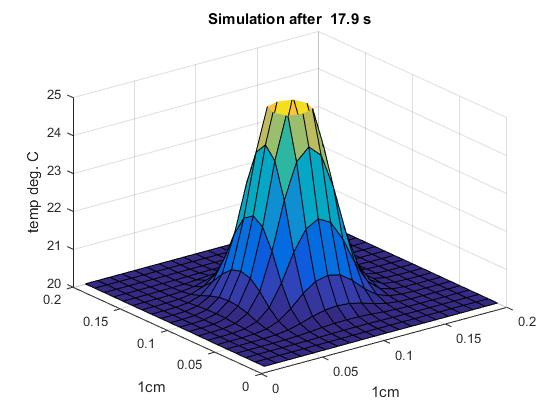
\includegraphics[scale=0.6]{first}}
\caption{Heat transfer for second boundary condition using copper plate after time}
\label{fig:plate}
\end{figure}

\begin{figure}[H]
\noindent\makebox[\textwidth]{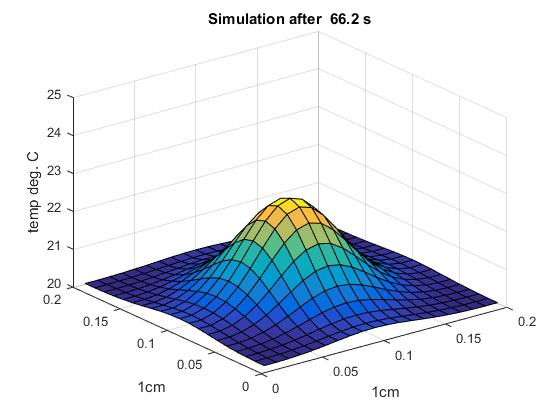
\includegraphics[scale=0.6]{second}}
\noindent\makebox[\textwidth]{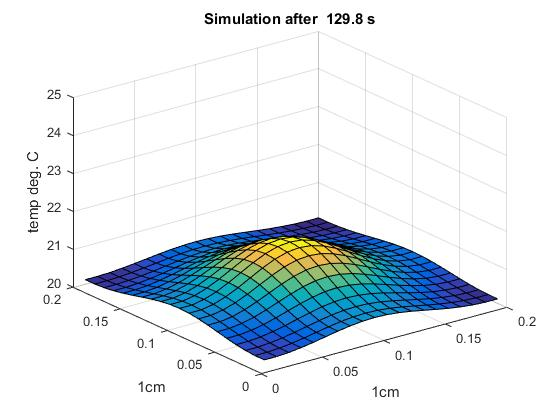
\includegraphics[scale=0.6]{third}}
\caption{Heat transfer for second boundary condition using copper plate after time}
\label{fig:plate}
\end{figure}
In both situations rapid temperature increase is observable nearby heater area. However in the second situation, much more dissipation can be observed.  After running such script against copper and alumina, it resolves that copper plate gives heat off much faster than alumina.

\subsection{Testing numerical stability}
System is numerically stable if small change in system property is resulting in small change to system behavior.
To test against numerical stability given model, \textit{binary-search-ish} algorithm is being used. Following code describes how it has been achieved.
\begin{lstlisting}[language=Matlab,frame=single,label={lst:autocorr},breaklines=true,caption={finding numerical stability point}]
% test for different dt values from 0.1 to 1.0
for i=0.1:0.1:1.0
    dt = i
    figure;
    % run simulation code
    tests;
    title(['dt = ' num2str(dt)]);
end
\end{lstlisting}
To find when system is starting to be unstable, output chart is being visually tested for evident oscillations. First iteration of this code gave result that oscillations are starting for dt between 0.2 and 0.3. To get more precise result, same code can be run with different iterator definition:
\begin{lstlisting}[language=Matlab,frame=single,label={lst:autocorr},breaklines=true,caption={iteration example}]
for i=0.2:0.01:0.3
   ...
\end{lstlisting}
and so on. After couple iterations, results came up as follows:
\begin{figure}[H]
\noindent\makebox[\textwidth]{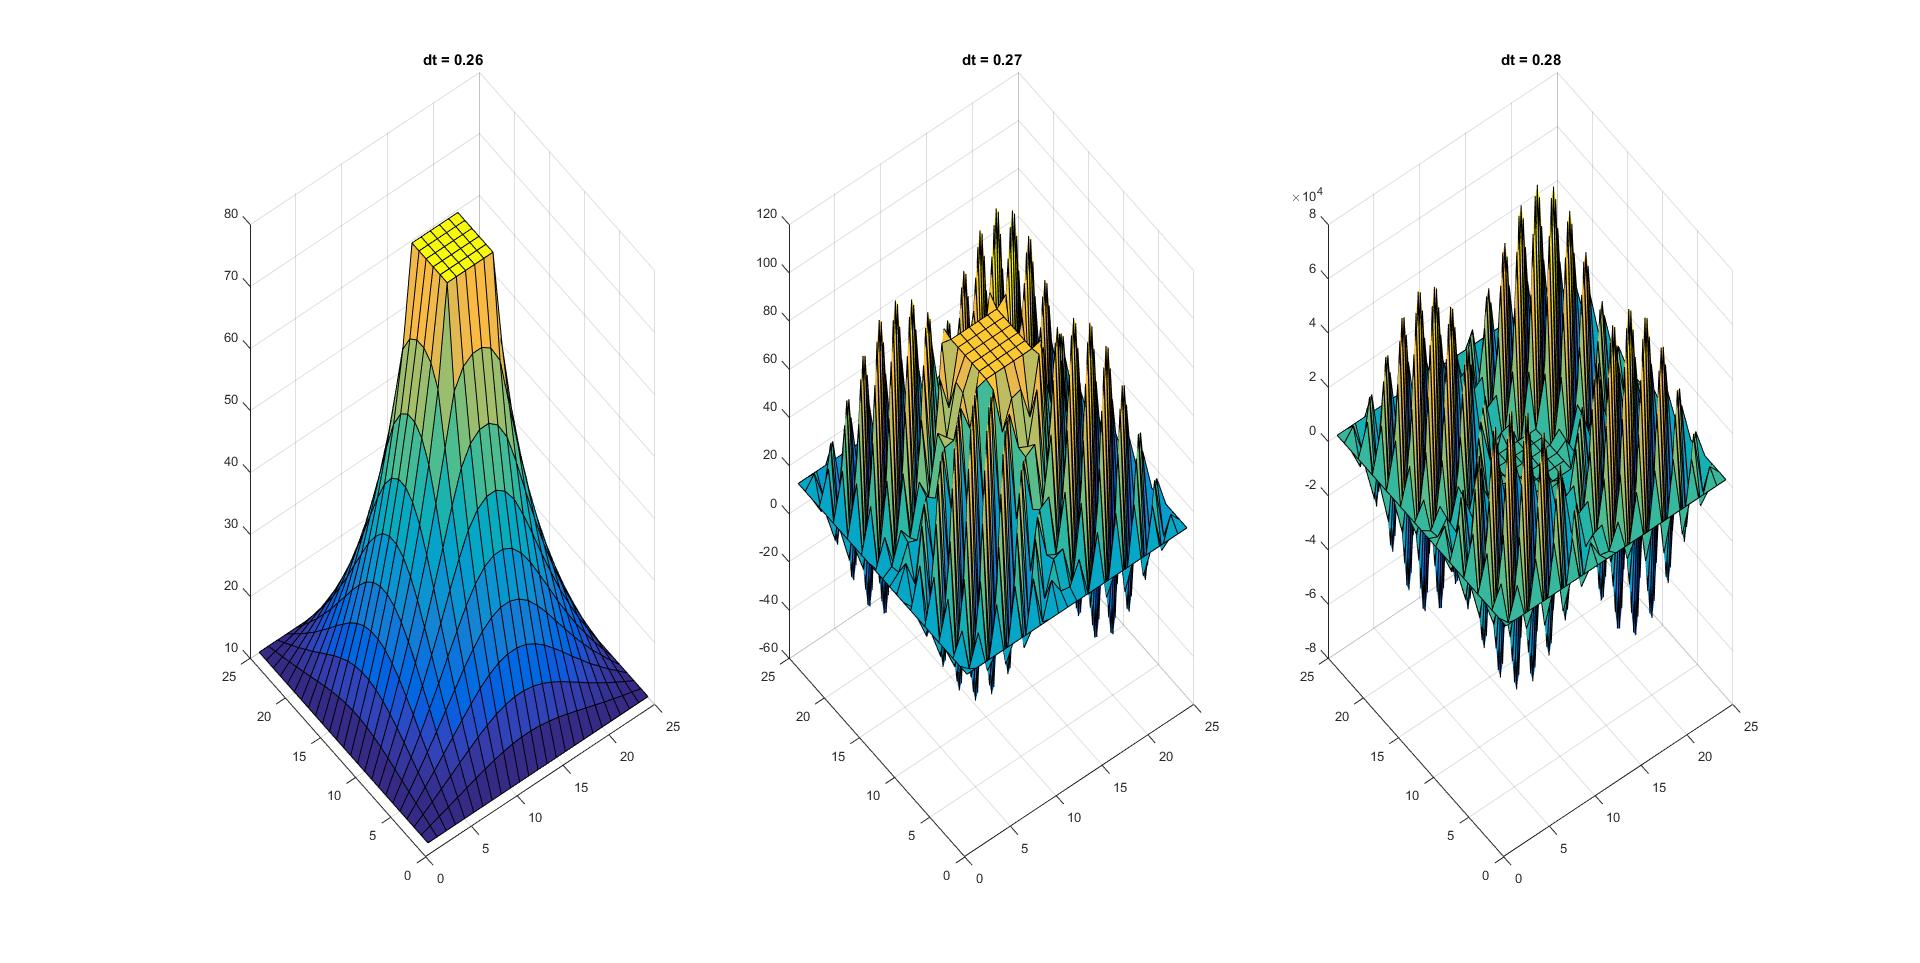
\includegraphics[scale=0.20]{numerical_stability}}
\caption{osculations for dt between 0.2s and 0.3s}
\label{fig:plate}
\end{figure}
Where it is clearly visible that system is loosing its stability somewhere between 0.26s and 0.28s for dt values.
Same thing can be done for spatial resolutions and the results came up as follows
\begin{figure}[H]
\noindent\makebox[\textwidth]{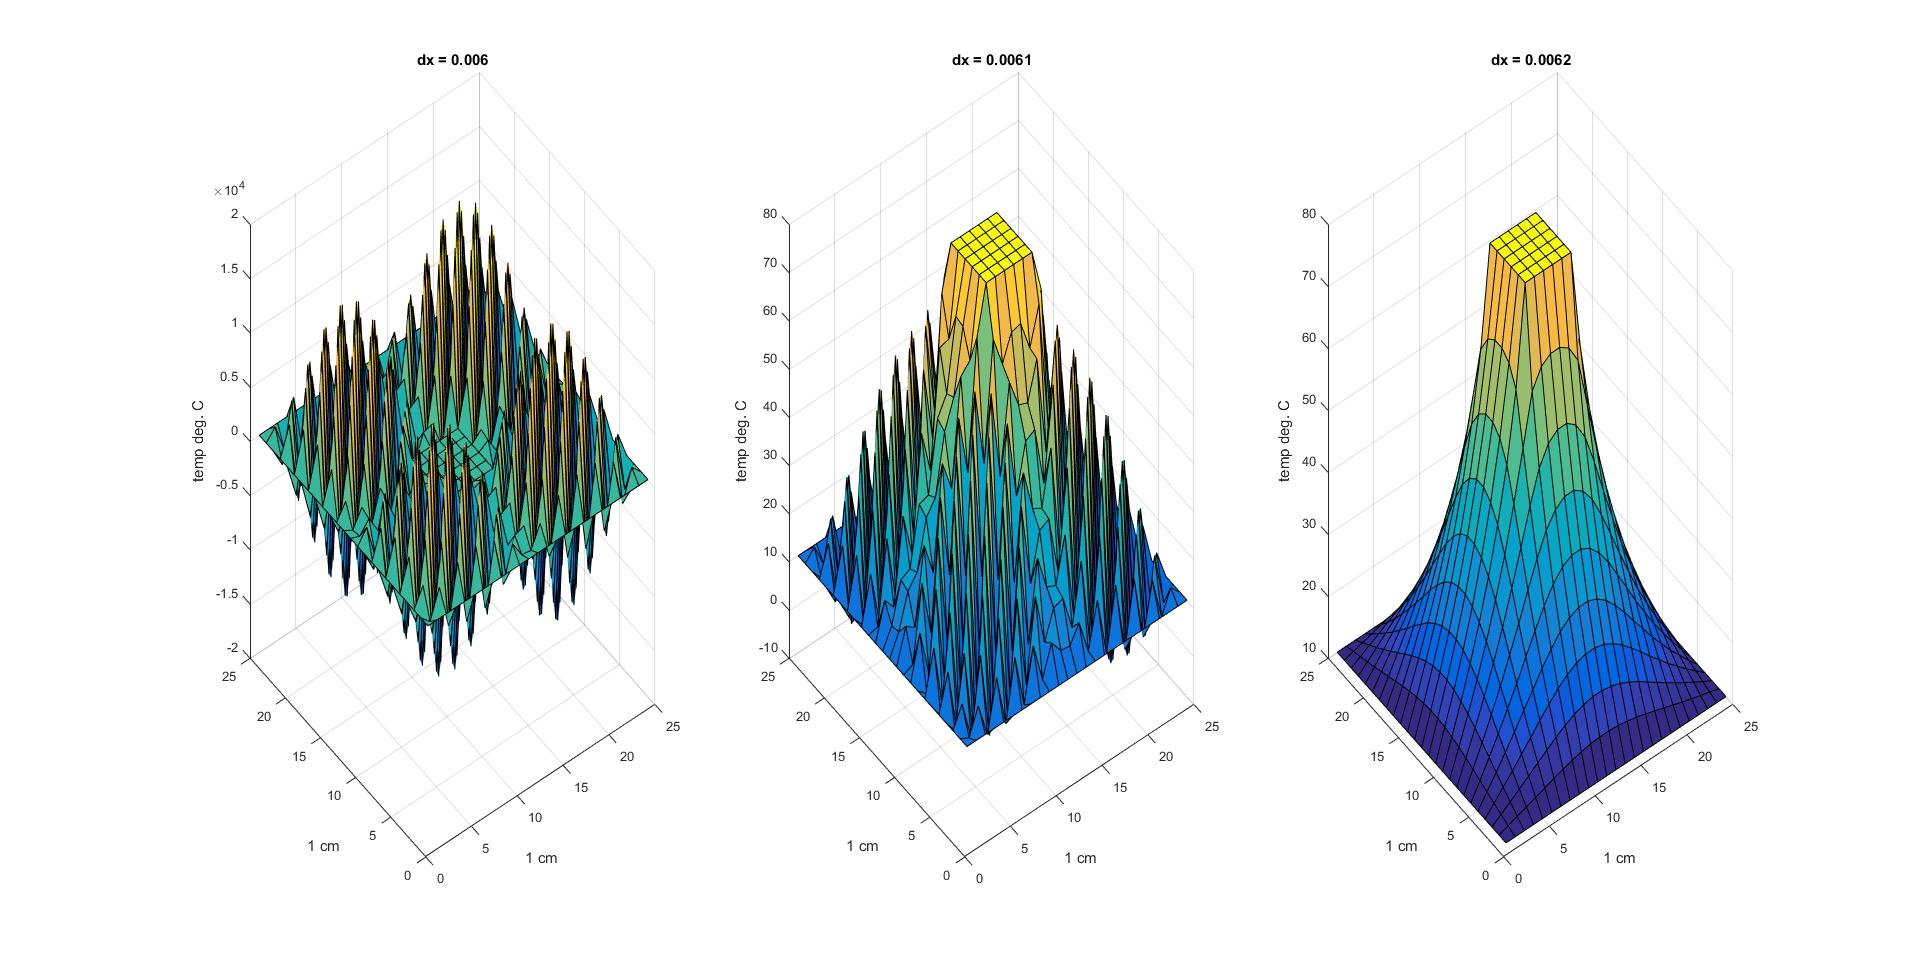
\includegraphics[scale=0.20]{spatial}}
\caption{osculations for dx between 0.0060m and 0.0062m}
\label{fig:plate}
\end{figure}
System is starting to osculate for $dx$ value between 0.0060 and 0,0062 m.

\subsection{Steady state calculation}
According to \textit{steady state} definition, system is in steady state when its properties are unchanging in time. In this case temperature change between time steps should be taken into consideration. Summing up, criterion for steady state of this system would be 
\begin{equation}
max(abs(system\_state\_matrix(i) - system\_state\_matrix(i-1))) = 0
\end{equation}.
However, because floating point numbers comparison is not so precise when it comes to programming languages, it is safe to assume that this equation shall be written like this:
\begin{equation}
max(abs(system\_state\_matrix(i) - system\_state\_matrix(i-1))) < \epsilon
\end{equation}
Where epsilon is some fixed value that is suitable in this case, i.e. $0.001^{o}C$. Given that formula, and adding it to code from listing \ref{lst:bc2}, it is testable when system reaches steady state:
\begin{lstlisting}[language=Matlab,frame=single,label={lst:autocorr},breaklines=true,caption={matlab snippet to find whether system is stable yet}]
    if (max(max(abs(plane(:,:,i) - plane(:,:,i-1))) < 0.001)) && (i * dt > 10)
        disp(i);
        break;
\end{lstlisting}
is resulting in i = 260, which corresponds to 26.0 seconds for copper and i = 1302, which is 130.2 seconds for alumina. Such result can be explained by very small $\epsilon$ value, which is fine in this case.

\subsection{Theory model vs simulation model}
This section purpose is to compare simulated temperature delta to calculated from stated formula:
\begin{equation}
\Delta T_T = \frac{P \cdot t_{heat}}{cw \cdot A^2 \cdot h \cdot \rho} = \frac{100W \cdot 10s}{900 \frac{J}{kgK} \cdot 0.25 m^2 \cdot 0.002m \cdot 2700 \frac{kg}{m3}} \approx 3.2922K
\end{equation}
To get $\Delta T$ from simulation model, following code can be executed
\begin{lstlisting}[language=Matlab,frame=single,label={lst:autocorr},breaklines=true,caption={Calculation of delta T in simulated heat transfer model for boundary condition 2}]
>> max(max(max(plane))) - start_temp
ans =

   8.0658
\end{lstlisting}
$\Delta T$ for theoretical model and simulation model is very different from each other. That means, that either equation is inaccurate (which is VERY unlikely) or the simulation parameters are a bit messed up (which is most probable). However, it is still same order of magnitude. That being said, it can be conclude that this result is acceptable.

\section{Conclusion}
In this report heat transfer and its properties was covered. Various matlab scripts were written to illustrate heat transfer itself, its relation to theoretical model and system stabilization property. This lab showed us that heat transfer phenomena can be simulated fairly easy however its accuracy in this implementation is something to think about. It is also worth mentioning that simulation of different materials is reasonably simple to achieve.
\end{document}
